\section{HSIC}
\label{sec:dep-hsic}

距离协方差用一种特定的权重比较特征函数，并且只适用于欧氏空间。第~\ref{chap:distribution-comparison}章的MMD给了比较两个分布的另一种通用办法：把分布映成再生核Hilbert空间中的核均值，再量两个核均值的距离。独立性问的正是两个分布$P_{(X,Y)}$与$P_X\otimes P_Y$是否相同，只要在乘积空间上选一个核，就能直接用MMD比较它们。

先回顾所用的记号。$k$是$\mathcal{X}$上的正定核，$\mathcal{H}_k$是它的RKHS。对满足$\mathbb{E}_{P}\sqrt{k(X,X)}<\infty$的分布$P$，核均值$m_P\in\mathcal{H}_k$由
\[
  \mathbb{E}_{P}[g(X)]=\langle g,m_P\rangle_{\mathcal{H}_k},\qquad g\in\mathcal{H}_k
\]
确定，取值为$m_P(y)=\mathbb{E}_{P}[k(X,y)]$。两个分布的MMD是两个核均值之差的范数$\lVert m_P-m_Q\rVert_{\mathcal{H}_k}$，记为$\operatorname{MMD}_k(P,Q)$，它等于$\mathcal{H}_k$单位球上期望差的最大值，平方可以写成核期望
\begin{equation}
  \operatorname{MMD}_k^{2}(P,Q)=\mathbb{E}\,k(U,U')-2\,\mathbb{E}\,k(U,V)+\mathbb{E}\,k(V,V'),
  \label{eq:dep-mmd-recall}
\end{equation}
其中$U,U'\sim P$，$V,V'\sim Q$，四者相互独立。若$P\mapsto m_P$是单射，称$k$为特征核，这时MMD为零当且仅当两个分布相同；欧氏空间上固定带宽的高斯核是特征核。

\subsection{联合分布的核比较}
\label{sec:dep-hsic-kernel-comparison}

在$\mathcal{X}$上取核$k$，在$\mathcal{Y}$上取核$l$。乘积空间$\mathcal{X}\times\mathcal{Y}$上最自然的核是两者的乘积
\[
  \kappa\bigl((x,y),(x',y')\bigr)=k(x,x')\,l(y,y'),
\]
称为\term{乘积核}（product kernel）。它仍是正定核：其Gram矩阵是两个Gram矩阵的逐元素乘积，正定性由Schur乘积定理保证，可参考\BookChapterRef{chap:rkhs}{卷四第23章“再生核Hilbert空间”}。本节假定$k,l$可测且有界，相应的RKHS可分，于是$\kappa$也有界，任何分布的核均值都存在。

\begin{definition}[HSIC]
\label{def:dep-hsic}
在上述条件下，$X$与$Y$关于核$k,l$的\term{Hilbert--Schmidt独立性准则}（Hilbert--Schmidt independence criterion），简称HSIC，定义为
\begin{equation}
  \operatorname{HSIC}_{k,l}(X,Y)=\operatorname{MMD}_{\kappa}^{2}\bigl(P_{(X,Y)},\,P_X\otimes P_Y\bigr).
  \label{eq:dep-hsic-def}
\end{equation}
\end{definition}

图~\ref{fig:dep-hsic-embedding}是这个定义的示意：两个分布各被送到$\mathcal{H}_\kappa$中的一个点，HSIC是这两点距离的平方。边缘乘积的核均值是$m_{P_X}$与$m_{P_Y}$的张量积：对独立的$\tilde{X}\sim P_X$、$\tilde{Y}\sim P_Y$，期望分解为
\[
  \mathbb{E}\bigl[k(\tilde{X},x)\,l(\tilde{Y},y)\bigr]=m_{P_X}(x)\,m_{P_Y}(y).
\]

\begin{BookInlineFigure}
  \centering
  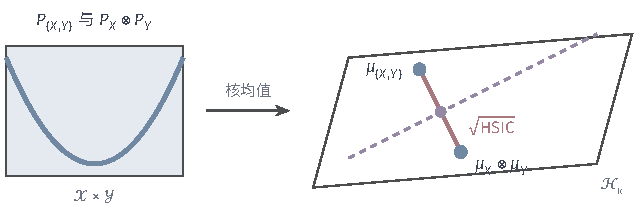
\includegraphics[width=107.9mm]{figures/07-probability/04-distribution-analysis/tikz/dep-hsic-embedding/figure.pdf}
  \caption{HSIC的几何图景。左：乘积空间上的两个分布，联合分布的质量集中在蓝色曲线上，边缘乘积摊在整个浅蓝矩形上。右：乘积核的RKHS$\mathcal{H}_\kappa$，两个核均值是两个蓝点，红色线段长度是$\sqrt{\operatorname{HSIC}}$。紫色虚线示意一个较贫乏的核只能看到的子空间：两个点在其上的投影（紫点）重合，这样的核给出零值。}
  \label{fig:dep-hsic-embedding}
\end{BookInlineFigure}

把式~\eqref{eq:dep-mmd-recall}用到这两个分布上，就得到只含核期望的表达。

\begin{theorem}[HSIC的核期望表示]
\label{thm:dep-hsic-expectation}
设$(X,Y)$、$(X',Y')$、$(X'',Y'')$相互独立且同分布。则
\begin{equation}
  \begin{aligned}
  \operatorname{HSIC}_{k,l}(X,Y)={}&\mathbb{E}\bigl[k(X,X')\,l(Y,Y')\bigr]+\mathbb{E}\bigl[k(X,X')\bigr]\,\mathbb{E}\bigl[l(Y,Y')\bigr]\\
  &-2\,\mathbb{E}\bigl[k(X,X')\,l(Y,Y'')\bigr].
  \end{aligned}
  \label{eq:dep-hsic-expectation}
\end{equation}
\end{theorem}

\begin{proof}
在式~\eqref{eq:dep-mmd-recall}中取$P=P_{(X,Y)}$，$Q=P_X\otimes P_Y$。第一项取$U=(X,Y)$，$U'=(X',Y')$，得$\mathbb{E}[k(X,X')l(Y,Y')]$。第三项中$V,V'$都服从边缘乘积，可以取$V=(X,Y'')$、$V'=(X',Y''')$，其中$Y'''$来自第四组独立复制；四个分量相互独立，期望分解为$\mathbb{E}[k(X,X')]\,\mathbb{E}[l(Y,Y')]$。第二项中$U=(X,Y)$，$V$服从边缘乘积且与$U$独立，取$V=(X',Y'')$，得到$\mathbb{E}[k(X,X')l(Y,Y'')]$。核有界，所有期望有限，代入即得。
\end{proof}

式~\eqref{eq:dep-hsic-expectation}与距离协方差的式~\eqref{eq:dep-dcov-pairwise}结构完全相同，只是把成对距离换成了核值。距离量的是“不相似”，核量的是“相似”，两者都在问：$X$这一对相似时，$Y$这一对是否也相似，超出边缘分布本身所能解释的程度。

\paragraph{中心化核}
与双重中心化同样，令
\[
  \tilde{k}(x,x')=k(x,x')-m_{P_X}(x)-m_{P_X}(x')+\mathbb{E}\,k(X,X'),
\]
称为\term{中心化核}（centered kernel），$\tilde{l}$类似。重复式~\eqref{eq:dep-dcov-centered}的验证（那里只用到中心化后对单个复制取期望为零），得到
\begin{equation}
  \operatorname{HSIC}_{k,l}(X,Y)=\mathbb{E}\bigl[\tilde{k}(X,X')\,\tilde{l}(Y,Y')\bigr].
  \label{eq:dep-hsic-centered}
\end{equation}
由再生性质展开可知，$\tilde{k}(x,x')$等于$k(x,\cdot)-m_{P_X}$与$k(x',\cdot)-m_{P_X}$在$\mathcal{H}_k$中的内积，就是把特征点平移到以核均值为原点后的内积。

\paragraph{交叉协方差算子}
HSIC这个名字来自另一种写法。对$f\in\mathcal{H}_k$、$g\in\mathcal{H}_l$，考虑$f(X)$与$g(Y)$的协方差。它对$f$、$g$都是线性的。由再生性质，$\lvert f(x)\rvert$不超过$\lVert f\rVert_{\mathcal{H}_k}\sqrt{k(x,x)}$，核有界时协方差被常数倍的$\lVert f\rVert\,\lVert g\rVert$控制。由Riesz表示定理，存在有界线性算子$\mathcal{C}_{XY}:\mathcal{H}_l\to\mathcal{H}_k$，使
\[
  \langle f,\mathcal{C}_{XY}\,g\rangle_{\mathcal{H}_k}=\operatorname{Cov}\bigl(f(X),g(Y)\bigr),
\]
称为\term{交叉协方差算子}（cross-covariance operator）。取$\mathcal{H}_k$与$\mathcal{H}_l$的规范正交基$\{e_i\}$、$\{e'_j\}$，HSIC等于这个算子的Hilbert--Schmidt范数的平方，
\begin{equation}
  \operatorname{HSIC}_{k,l}(X,Y)=\sum_{i,j}\operatorname{Cov}\bigl(e_i(X),\,e'_j(Y)\bigr)^{2}.
  \label{eq:dep-hsic-operator}
\end{equation}

式~\eqref{eq:dep-hsic-operator}可以从式~\eqref{eq:dep-hsic-centered}推出。记$\tilde{e}_i(x)=e_i(x)-\mathbb{E}e_i(X)$，由再生性质它等于$e_i$与$k(x,\cdot)-m_{P_X}$的内积。由Parseval等式，
\[
  \sum_i\tilde{e}_i(x)\,\tilde{e}_i(x')=\bigl\langle k(x,\cdot)-m_{P_X},\,k(x',\cdot)-m_{P_X}\bigr\rangle=\tilde{k}(x,x'),
\]
$\tilde{l}$同样展开。部分和由Cauchy--Schwarz不等式被$\lVert k(x,\cdot)-m_{P_X}\rVert\lVert k(x',\cdot)-m_{P_X}\rVert$控制，核有界时这是常数，可以用支配收敛定理交换求和与期望：
\[
  \mathbb{E}\bigl[\tilde{k}(X,X')\tilde{l}(Y,Y')\bigr]=\sum_{i,j}\mathbb{E}\bigl[\tilde{e}_i(X)\tilde{e}'_j(Y)\bigr]\,\mathbb{E}\bigl[\tilde{e}_i(X')\tilde{e}'_j(Y')\bigr].
\]
两组复制独立，每个乘积因子都是$\operatorname{Cov}(e_i(X),e'_j(Y))$，即得式~\eqref{eq:dep-hsic-operator}。

这个写法给出了直观：HSIC同时检查无穷多对特征函数$e_i(X)$、$e'_j(Y)$之间的协方差，把它们的平方加起来。协方差只检查一对线性函数；核越丰富，被检查的函数对越多。

\paragraph{线性核只剩协方差}
取最贫乏的核，$\mathcal{X}=\mathcal{Y}=\mathbb{R}$上的线性核$k(x,x')=xx'$、$l(y,y')=yy'$。它们无界，但当$X,Y$有二阶矩时式~\eqref{eq:dep-hsic-expectation}的各项仍然有限。代入，
\[
  \begin{aligned}
  &\mathbb{E}[XX'YY']+\mathbb{E}[XX']\,\mathbb{E}[YY']-2\,\mathbb{E}[XX'YY'']\\
  &\qquad=(\mathbb{E}XY)^{2}+(\mathbb{E}X)^{2}(\mathbb{E}Y)^{2}-2\,\mathbb{E}XY\,\mathbb{E}X\,\mathbb{E}Y ,
  \end{aligned}
\]
右边正是$\operatorname{Cov}(X,Y)^{2}$。线性核的RKHS只含线性函数，式~\eqref{eq:dep-hsic-operator}只剩一项。三点抛物线和连续抛物线在线性核下HSIC都是零。

\paragraph{距离诱导核}
距离协方差也是一个HSIC，只是用的核无界。在$\mathbb{R}^{d}$上令
\[
  k_{\mathrm{d}}(\bm{x},\bm{x}')=\tfrac12\bigl(\lVert\bm{x}\rVert_2+\lVert\bm{x}'\rVert_2-\lVert\bm{x}-\bm{x}'\rVert_2\bigr),
\]
称为\term{距离诱导核}（distance-induced kernel）。

它是正定的。由引理~\ref{lem:dep-cos-integral}，$k_{\mathrm{d}}$的三项各写成$1-\cos$的积分。记$\alpha=\langle\bm{t},\bm{x}\rangle$，$\beta=\langle\bm{t},\bm{x}'\rangle$，展开右边的乘积可以验证
\[
  \begin{aligned}
  &(1-\cos\alpha)+(1-\cos\beta)-\bigl(1-\cos(\alpha-\beta)\bigr)\\
  &\qquad=\operatorname{Re}\bigl[(\mathrm{e}^{\mathrm{i}\alpha}-1)\,\overline{(\mathrm{e}^{\mathrm{i}\beta}-1)}\bigr].
  \end{aligned}
\]
记
\[
  g_{\bm{x}}(\bm{t})=\mathrm{e}^{\mathrm{i}\langle\bm{t},\bm{x}\rangle}-1 .
\]

把三项的积分合并，得到
\[
  k_{\mathrm{d}}(\bm{x},\bm{x}')=\frac{1}{2c_d}\int_{\mathbb{R}^{d}}\frac{\operatorname{Re}\bigl[g_{\bm{x}}(\bm{t})\overline{g_{\bm{x}'}(\bm{t})}\bigr]}{\lVert\bm{t}\rVert_2^{d+1}}\,\mathrm{d}\bm{t},
\]
这是一个加权$L^{2}$内积的实部。对任意点$\bm{x}_1,\dots,\bm{x}_n$与实数$c_1,\dots,c_n$，
\[
  \sum_{i,j}c_ic_j\,k_{\mathrm{d}}(\bm{x}_i,\bm{x}_j)=\frac{1}{2c_d}\int_{\mathbb{R}^{d}}\frac{\bigl\lvert\sum_ic_ig_{\bm{x}_i}(\bm{t})\bigr\rvert^{2}}{\lVert\bm{t}\rVert_2^{d+1}}\,\mathrm{d}\bm{t}\geq0 .
\]

$k_{\mathrm{d}}$中的$\lVert\bm{x}\rVert_2$与$\lVert\bm{x}'\rVert_2$只依赖一个端点，在中心化中被消去，所以$\tilde{k}_{\mathrm{d}}=-\frac12A$，$A$是式~\eqref{eq:dep-double-centering}的双重中心化距离。代入式~\eqref{eq:dep-hsic-centered}与式~\eqref{eq:dep-dcov-centered}，在二阶矩有限时
\[
  \operatorname{HSIC}_{k_{\mathrm{d}},l_{\mathrm{d}}}(\bm{X},\bm{Y})=\tfrac14\operatorname{dCov}^{2}(\bm{X},\bm{Y}).
\]
距离协方差因此是HSIC的一个特例。核无界时，HSIC的每一项能否积分要另外检查，这里所需的正是二阶矩。

\paragraph{两个手算例子}
标准二元高斯在高斯核下有闭式。取$k(x,x')=\exp(-(x-x')^{2}/2)$，$l$相同（带宽$1$）。式~\eqref{eq:dep-hsic-expectation}的每一项都形如$\mathbb{E}\exp(-\frac12(U^{2}+V^{2}))$，其中$(U,V)$是均值为零的二元高斯，协方差矩阵记为$\bm{S}$。把高斯密度代入并配方，
\[
  \mathbb{E}\exp\Bigl(-\tfrac12(U^{2}+V^{2})\Bigr)=\frac{1}{2\pi\sqrt{\det\bm{S}}}\int_{\mathbb{R}^{2}}\mathrm{e}^{-\frac12\bm{w}^{\top}(\bm{S}^{-1}+\bm{I})\bm{w}}\,\mathrm{d}\bm{w}=\det(\bm{I}+\bm{S})^{-1/2}.
\]
三项分别对应$(U,V)=(X-X',Y-Y')$、两者独立、$(X-X',Y-Y'')$，协方差矩阵的对角元都是$2$，非对角元分别为$2\rho$、$0$、$\rho$。$\det(\bm{I}+\bm{S})$依次为$9-4\rho^{2}$、$9$、$9-\rho^{2}$，于是
\begin{equation}
  \operatorname{HSIC}=\frac{1}{\sqrt{9-4\rho^{2}}}+\frac13-\frac{2}{\sqrt{9-\rho^{2}}}.
  \label{eq:dep-hsic-gauss}
\end{equation}
$\rho=0.5$时三项为$0.35355$、$0.33333$、$-0.67612$，
\[
  \operatorname{HSIC}\approx0.35355+0.33333-0.67612=0.01076 .
\]

三点抛物线在同样的核下是有限和。记$\alpha=\mathrm{e}^{-1/2}\approx0.6065$，$\beta=\mathrm{e}^{-2}\approx0.1353$，三个点按$x=-1,0,1$排列，核矩阵为
\[
  \bm{K}=\begin{pmatrix}1&\alpha&\beta\\ \alpha&1&\alpha\\ \beta&\alpha&1\end{pmatrix},\qquad
  \bm{L}=\begin{pmatrix}1&\alpha&1\\ \alpha&1&\alpha\\ 1&\alpha&1\end{pmatrix}.
\]
式~\eqref{eq:dep-hsic-expectation}的三项分别是$\frac19\sum_{i,j}K_{i,j}L_{i,j}$、两个矩阵各自的元素平均之积、以及$\frac13\sum_i\bar{K}_i\bar{L}_i$（$\bar{K}_i,\bar{L}_i$为第$i$行的平均）。数值为
\[
  \begin{gathered}
  \mathbb{E}[kl]\approx0.52691,\qquad \mathbb{E}[kl'']\approx0.51771,\\
  \mathbb{E}[k]\,\mathbb{E}[l]\approx0.63298\times0.82512\approx0.52228,
  \end{gathered}
\]
所以$\operatorname{HSIC}\approx0.52691+0.52228-2\times0.51771\approx0.01378$。

\subsection{零值判据与核选择}
\label{sec:dep-hsic-zero}

由定义~\ref{def:dep-hsic}，HSIC为零当且仅当两个核均值相同。核均值能否分辨$P_{(X,Y)}$与$P_X\otimes P_Y$，取决于乘积核$\kappa$。

\begin{theorem}[HSIC的零值判据]
\label{thm:dep-hsic-zero}
若乘积核$\kappa=k\otimes l$在$\mathcal{X}\times\mathcal{Y}$的概率分布上是特征核，则
\begin{equation}
  \operatorname{HSIC}_{k,l}(X,Y)=0\iff X\text{与}Y\text{独立}.
  \label{eq:dep-hsic-zero}
\end{equation}
特别地，$\mathcal{X}=\mathbb{R}^{p}$、$\mathcal{Y}=\mathbb{R}^{q}$，$k,l$为带宽$\sigma,\tau>0$的高斯核时，结论成立。
\end{theorem}

\begin{proof}
式~\eqref{eq:dep-hsic-zero}是特征核的定义：MMD为零当且仅当两个分布相同。对高斯核，乘积核为
\[
  \kappa\bigl((\bm{x},\bm{y}),(\bm{x}',\bm{y}')\bigr)=\exp\Bigl(-\frac{\lVert\bm{x}-\bm{x}'\rVert_2^{2}}{2\sigma^{2}}-\frac{\lVert\bm{y}-\bm{y}'\rVert_2^{2}}{2\tau^{2}}\Bigr).
\]
作线性变换$T(\bm{x},\bm{y})=(\bm{x}/\sigma,\bm{y}/\tau)$，则$\kappa(\bm{z},\bm{z}')=k_1(T\bm{z},T\bm{z}')$，$k_1$是$\mathbb{R}^{p+q}$上带宽为$1$的高斯核。若两个分布$P,Q$的$\kappa$核均值相同，则推前分布$T_{\#}P$与$T_{\#}Q$的$k_1$核均值相同；$k_1$是特征核，所以$T_{\#}P=T_{\#}Q$，$T$可逆，于是$P=Q$。
\end{proof}

若$\sigma=\tau$，把第~\ref{chap:distribution-comparison}章高斯核MMD的谱表示用到$\mathbb{R}^{p+q}$上，HSIC就是$\lvert\Delta(\bm{t},\bm{s})\rvert^{2}$对高斯分布$\mathcal{N}(\bm{0},\sigma^{-2}\bm{I})$的积分。它与距离协方差的定义~\eqref{eq:dep-dcov-def}只差权重：高斯权重是可积的概率密度，不需要矩条件，但强烈压低高频；距离协方差的幂次权重不可积，换来了与距离的对应和尺度上的等变性。

特征核是充分条件。对欧氏空间上的平移不变核，已知只要$k$与$l$各自是特征核，HSIC的零值就刻画独立\scite{math-gretton2015hsic}。核不够丰富时，HSIC为零只说明它所检查的那些函数对的协方差都为零，例如线性核下只说明不相关。图~\ref{fig:dep-hsic-embedding}中紫色虚线表示的正是这种情况。

\paragraph{核尺度改变数值}
高斯核的带宽决定了HSIC“在多大尺度上看”。带宽很小时，核只在几乎重合的点对上取值接近$1$，连续分布下各项都趋于零；带宽很大时，在数据范围内$k(x,x')\approx1-(x-x')^{2}/(2\sigma^{2})$，核近似退化为常数加二次项，HSIC按$\sigma^{-4}$趋于零，并且主要反映协方差。中间某个尺度上HSIC最大。

图~\ref{fig:dep-hsic-bandwidth}对比两个分布：$\rho=0.5$的标准二元高斯（式~\eqref{eq:dep-hsic-gauss}的推广）与连续抛物线（数值积分），两个坐标用相同带宽$s$。抛物线的取值范围小，在$s\approx0.19$处达到最大值约$0.067$；高斯在$s\approx0.95$处达到约$0.0108$。两条曲线在$s\approx0.7$与$0.78$之间相交：带宽小于此时抛物线的HSIC更大，大于此时高斯的更大。$s=1$时两者分别为$0.0108$与$0.0026$。

\begin{BookInlineFigure}
  \centering
  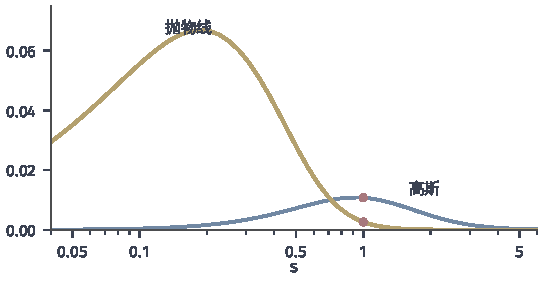
\includegraphics[width=92mm]{figures/07-probability/04-distribution-analysis/matplotlib/dep-hsic-bandwidth/figure.pdf}
  \caption{高斯核HSIC随带宽$s$的变化（横轴为对数刻度，两个坐标用同一带宽）。蓝线：$\rho=0.5$的标准二元高斯，闭式计算；黄线：$X\sim\operatorname{Unif}(-1,1)$、$Y=X^{2}$，对$X$取$1000$个节点数值积分。红点为$s=1$处的$0.0108$与$0.0026$。两条曲线在$s\approx0.74$附近相交。}
  \label{fig:dep-hsic-bandwidth}
\end{BookInlineFigure}

所以“这个分布的HSIC比那个大”只有在指定了核与带宽以后才有意义；换一个带宽，次序可以颠倒。不同核下的HSIC数值不在同一个刻度上，不能直接比较。把HSIC除以$\sqrt{\operatorname{HSIC}_{k,k}(X,X)\operatorname{HSIC}_{l,l}(Y,Y)}$可以得到与距离相关类似的归一化量，它消去了一部分尺度影响，但仍依赖带宽。根据样本选带宽的经验规则涉及估计问题，不在本章讨论。
